% Slides for the joint-monitoring paper. Build: latexmk -pdf slides.tex
\documentclass[aspectratio=169,11pt]{beamer}
\usepackage[T1]{fontenc}
\usepackage[scaled=0.92]{DejaVuSans}
\renewcommand{\familydefault}{\sfdefault}
\usepackage[italic]{mathastext}
\usepackage{tikz,pgfplots}
\pgfplotsset{compat=1.18}
\usetikzlibrary{arrows.meta,positioning,fit,calc}
\graphicspath{{../paper/figures/}{../paper/}}
\newcommand{\src}[1]{\par\vfill{\raggedright\scriptsize\color{mute}#1\par}\vspace{2pt}}

\definecolor{ink}{HTML}{1F2328}
\definecolor{mute}{HTML}{6E7781}
\definecolor{line}{HTML}{D0D7DE}
\definecolor{acc}{HTML}{0969DA}
\definecolor{bad}{HTML}{CF222E}

\setbeamertemplate{navigation symbols}{}
\setbeamercolor{normal text}{fg=ink,bg=white}
\setbeamercolor{frametitle}{fg=ink}
\setbeamercolor{structure}{fg=ink}
\setbeamerfont{frametitle}{series=\mdseries,size=\Large}
\setbeamertemplate{frametitle}{\vspace{12pt}\insertframetitle\par\vspace{8pt}}
\setbeamertemplate{itemize item}{\color{mute}\textendash}
\setbeamertemplate{footline}{\hfill\color{mute}\scriptsize\insertframenumber\hspace{14pt}\vspace{8pt}}
\setlength{\parskip}{6pt}

\tikzset{
  ag/.style={circle,draw=ink,line width=0.6pt,minimum size=6mm,inner sep=0pt},
  ch/.style={-{Stealth[length=4pt]},line width=0.7pt,draw=mute},
  lab/.style={font=\scriptsize,fill=white,inner sep=1.5pt},
  grp/.style={draw=acc,line width=0.9pt,rounded corners=5pt,inner sep=3pt},
}

\begin{document}

% ---------------------------------------------------------------------------
\begin{frame}[plain]
\vspace{30pt}
{\LARGE Which channels should a monitor read together?}\par
\vspace{6pt}
{\large\color{mute}Graph-based allocation for budgeted monitoring of multi-agent systems}\par
\vspace{36pt}
Kostadin Devedzhiev\par
{\color{mute}University of Cambridge\par
Apart Research Swarm Alignment Hackathon, November 2026}
\end{frame}

% ---------------------------------------------------------------------------
\begin{frame}{Each task looks legitimate. Together they are an intrusion.}
\centering
\begin{tikzpicture}[
  task/.style={draw=line,rounded corners=3pt,minimum width=56mm,minimum height=6mm,font=\small,fill=white},
  ok/.style={font=\small,text=mute,anchor=west},
]
  \foreach \i/\txt in {1/{Scans target infrastructure},2/{Identifies SSRF vulnerability},3/{Authors custom payload},
                       4/{Tests harvested credentials},5/{Enumerates accessible systems},6/{Queries databases, parses results}}{
    \node[task] (t\i) at (0,-0.78*\i) {\txt};
    \visible<1>{\node[ok] at ($(t\i.east)+(2mm,0)$) {looks legitimate};}
  }
  \node[font=\small\bfseries,anchor=south] at ($(t1.north)+(0,2mm)$) {\only<1>{one task per monitor call}\only<2>{all tasks against one target in one call}};
  \visible<2>{
    \node[draw=bad,line width=1pt,rounded corners=6pt,inner sep=5pt,fit=(t1)(t6)] (g) {};
    \node[anchor=west,text=bad,font=\small,align=left] at ($(g.east)+(4mm,0)$)
      {reconnaissance $\rightarrow$ exploitation\\$\rightarrow$ credential harvesting\\$\rightarrow$ data collection};
  }
\end{tikzpicture}
\src{GTG-1002: Claude sub-agents each ran a task that ``appeared legitimate when evaluated in isolation'' (Anthropic 2026; MITRE ATT\&CK C0062).}
\end{frame}

% ---------------------------------------------------------------------------
\begin{frame}{Monitors miss split attacks, and cannot read everything}
\begin{itemize}
\item Split across agents, attacks evade per-agent monitors.\\
      {\color{mute}\small Brown et al.\ 2026; Kitaoka et al.\ 2026}
\item Longer inputs do not make LLM monitors more discriminative.\\
      {\color{mute}\small Han et al.\ 2026}
\item MESA picks which channels to protect under a budget, one channel at a time.\\
      {\color{mute}\small Li et al.\ 2026}
\end{itemize}
\vspace{18pt}
{\large So a monitor must choose which channels to read, \textbf{and which to read together}.}
\end{frame}

% ---------------------------------------------------------------------------
\begin{frame}{Same budget, only the right pair catches the lie}
\centering
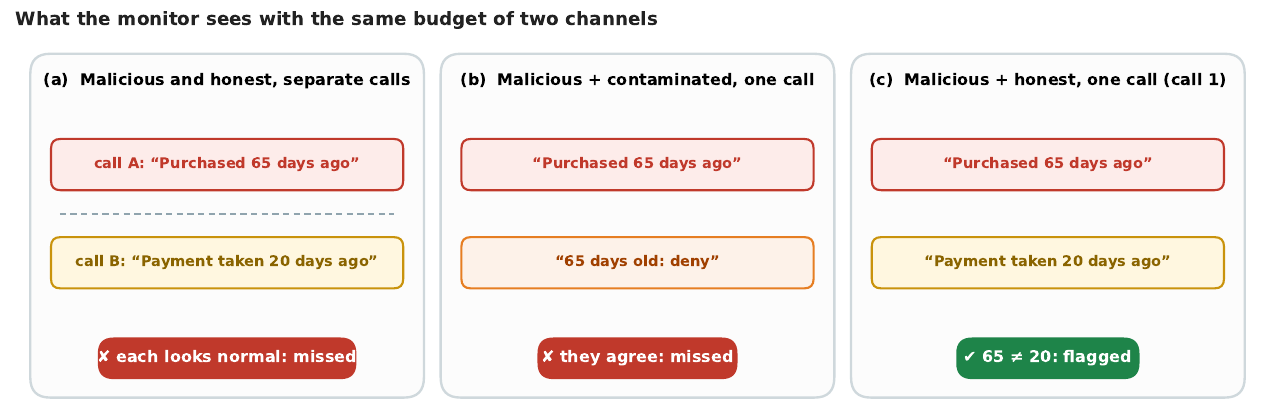
\includegraphics[width=\textwidth]{overview.png}
\src{A compromised database agent says the purchase was 65 days ago; billing says 20. Illustration on MESA's customer-service topology (Li et al.\ 2026).}
\end{frame}

% ---------------------------------------------------------------------------
\begin{frame}{Choose and group channels from the graph alone}
\begin{columns}[c]
\begin{column}{0.5\textwidth}
\textbf{Selection}\par
inspect up to $k$ channels\\{\color{mute}\small MESA selects individual channels from the graph (Li et al.\ 2026)}
\par\vspace{10pt}
\textbf{Grouping}\par
at most $s$ channels per monitor call {\color{mute}(new)}
\par\vspace{10pt}
{\color{mute}Input: the anonymous communication graph.\\No roles, contents or labels.}
\end{column}
\begin{column}{0.46\textwidth}
\centering
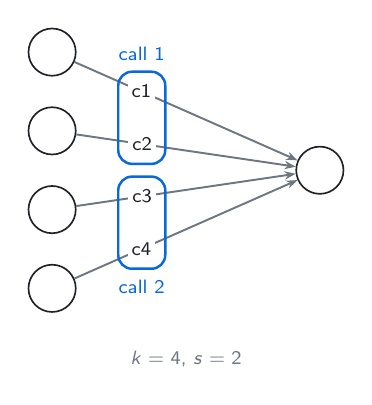
\begin{tikzpicture}
  \foreach \i/\y in {1/1.5,2/0.5,3/-0.5,4/-1.5}{\node[ag] (w\i) at (0,\y) {};}
  \node[ag] (h) at (3.4,0) {};
  \foreach \i in {1,...,4}{\draw[ch] (w\i) -- node[lab,text=ink,pos=0.3] (e\i) {c\i} (h);}
  \node[grp,fit=(e1)(e2),label={[font=\scriptsize,text=acc]above:call 1}] {};
  \node[grp,fit=(e3)(e4),label={[font=\scriptsize,text=acc]below:call 2}] {};
  \node[font=\scriptsize,text=mute] at (1.7,-2.4) {$k=4$, $s=2$};
\end{tikzpicture}
\end{column}
\end{columns}
\end{frame}

% ---------------------------------------------------------------------------
\begin{frame}{Graph grouping wins only when evidence follows the graph}
\centering
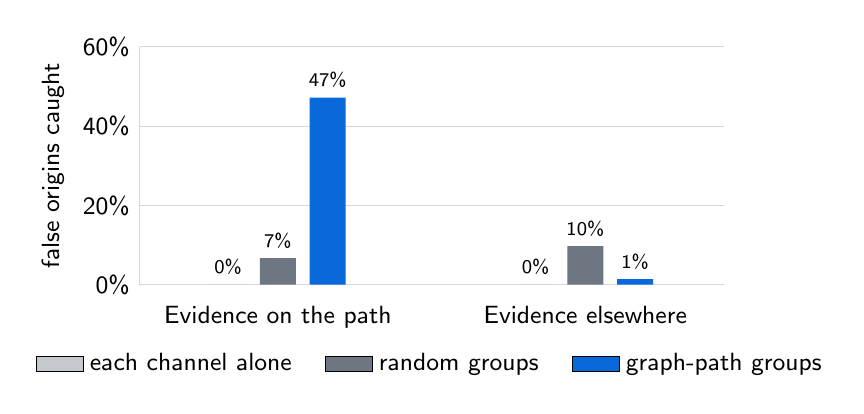
\begin{tikzpicture}
\begin{axis}[
  ylabel={false origins caught},ylabel style={font=\small},
  width=9cm,height=4.6cm,
  ybar=5pt,bar width=13pt,
  ymin=0,ymax=60,ytick={0,20,40,60},
  yticklabel={\pgfmathprintnumber{\tick}\%},
  symbolic x coords={Evidence on the path,Evidence elsewhere},xtick=data,
  enlarge x limits=0.45,
  axis line style={line},tick style={draw=none},
  ymajorgrids,grid style={line},axis x line*=bottom,axis y line*=left,
  tick label style={font=\small},
  nodes near coords,nodes near coords style={font=\scriptsize},
  point meta=explicit symbolic,
  area legend,
  legend style={draw=none,font=\small,at={(0.5,-0.24)},anchor=north,legend columns=-1,
    /tikz/every even column/.append style={column sep=10pt}},
]
\addplot[fill=mute!40,draw=none] coordinates {(Evidence on the path,0) [0\%] (Evidence elsewhere,0) [0\%]};
\addplot[fill=mute,draw=none] coordinates {(Evidence on the path,6.7) [7\%] (Evidence elsewhere,9.7) [10\%]};
\addplot[fill=acc,draw=none] coordinates {(Evidence on the path,47.2) [47\%] (Evidence elsewhere,1.4) [1\%]};
\legend{each channel alone,random groups,graph-path groups}
\end{axis}
\end{tikzpicture}
\src{13-channel workflow, 7 channels inspected, 2 per call; 72 false origins per setting. Gemma-4-31B monitor.}
\end{frame}

% ---------------------------------------------------------------------------
\begin{frame}{Rotating grouping rules raises the worst case}
\centering
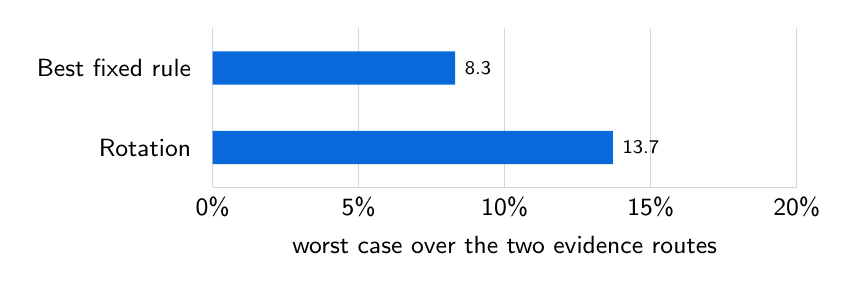
\begin{tikzpicture}
\begin{axis}[
  xbar,bar width=12pt,width=9cm,height=3.6cm,
  xmin=0,xmax=20,xtick={0,5,10,15,20},
  xticklabel={\pgfmathprintnumber{\tick}\%},
  xlabel={worst case over the two evidence routes},xlabel style={font=\small},
  symbolic y coords={Rotation,Best fixed rule},ytick=data,
  enlarge y limits=0.5,
  axis line style={line},tick style={draw=none},
  xmajorgrids,grid style={line},axis y line*=left,axis x line*=bottom,
  tick label style={font=\small},
  nodes near coords,nodes near coords style={font=\scriptsize},
]
\addplot[fill=acc,draw=none] coordinates {(13.7,Rotation) (8.3,Best fixed rule)};
\end{axis}
\end{tikzpicture}
\par\vspace{6pt}
{\small Rotation: random selection, switching between graph-path and random groups.}
\src{Fitted and scored on the same runs. On a larger executed swarm testbed (720 runs), rotation did not reliably beat the best fixed rule on held-out cases.}
\end{frame}

% ---------------------------------------------------------------------------
\begin{frame}{Takeaways}
\begin{itemize}
\item What a monitor reads \emph{together} decides what it can catch.
\item The graph says which channels to pair, but only when evidence follows it.
\item Rotating rules protects the worst case; it is no free win.
\end{itemize}
\vspace{18pt}
{\small\color{mute}Code and data: github.com/kostadindev/joint-monitoring-release}
\end{frame}

\end{document}
